\documentclass[10pt]{article}

\usepackage{titling}
\usepackage{titlesec}
\usepackage{geometry}
\usepackage{setspace}
\usepackage{float}
\usepackage{graphicx}
\usepackage[font=small,labelfont=bf]{caption}
\geometry{margin=.75in}
\setstretch{1.05}
\setlength{\droptitle}{-1.2cm}
\setlength{\textfloatsep}{0.7em}
\setlength{\floatsep}{0.4em}
\setlength{\intextsep}{0.4em}

\setlength{\abovecaptionskip}{0.4em}
\setlength{\belowcaptionskip}{0.2em}
\setstretch{0.95}


\titlespacing*{\section}{0pt}{0.8em}{0.4em}
\titlespacing*{\subsection}{0pt}{0.6em}{0.3em}

\makeatletter
\renewcommand{\maketitle}{
  \begin{center}
    {\Large \@title \par}
    \vskip 0.25em
    {\small \@author \par}
    {\footnotesize \@date \par}
  \end{center}
}
\makeatother

\title{Temporal Structure of Response Behavior in an AI Java Tutor}
\author{\small Anissa Williams \\ \small DAT 507: Scientific Computing}
\date{\footnotesize April 2026}



\begin{document}
\maketitle

\begin{abstract}
AI tutoring systems generate detailed logs of student interactions, including timestamps for every message. These logs contain a rich temporal signal that reflects how students behave during learning. This project analyzes the structure of student response times in an AI-guided Java tutoring system using numerical and time-series methods as a way of characterizing interaction rhythm and engagement dynamics. The goal is to understand how pacing, momentum, variability, and frequency structure differ across instructional designs. The analysis focuses on three tutoring conditions: Character-Scaffolded, Non-Character Scaffolded, and Direct Chat. Results show that scaffolded sessions exhibit faster responses, negative within-session slopes, and multi-frequency rhythmic structure, while direct chat sessions slow down and display a single dominant low-frequency trend. These findings demonstrate that response times alone contain meaningful behavioral information about student engagement.
\end{abstract}

\section{Introduction}


Artificial Intelligence in Education (AIED) has increasingly focused on adaptive systems that personalize instruction and provide timely feedback. A central goal in this domain is the early identification of students at risk of poor learning outcomes, enabling intervention \textit{during} the learning process rather than \textit{after} assessment.

Recent advances in large language models (LLMs) have introduced conversational AI tutors that interact with students in natural language. These systems generate fine-grained interaction logs, capturing not only what students say, but how they engage over time. These logs don’t just capture what students say; they show how the interaction \textit{unfolds}, including timing, pacing, and the structure of the back‑and‑forth.

While prior work has shown that aggregate measures such as total messages or time-on-task correlate with performance, \cite{papadogiannis2024} these metrics do not capture how engagement unfolds during a session. Two students may spend similar amounts of time interacting with a tutor yet exhibit very different patterns of behavior: one steady and deliberate, the other irregular and bursty.

This paper proposes a \textit{behavioral rhythm} framework for analyzing student interaction patterns in AI tutoring systems. In this context, rhythm refers to the temporal structure of interaction, including the consistency, pacing, and distribution of responses over time. Rather than focusing solely on the quantity of engagement, this approach shifts the focus from how much students engage to how that engagement is organized temporally.

Using a controlled dataset of conversational logs from a university-level Java tutoring study, we examine whether rhythm-based features provide insight into student performance. We show that interaction rhythm captures meaningful differences in learning behavior and complements traditional engagement metrics, offering a more interpretable view of how students interact with AI tutors.

\section{Dataset and Preprocessing}

The dataset contains 115 completed tutoring sessions, 2,874 total messages, and 1,381 user messages. Each message includes a timestamp, allowing construction of per-session response-time sequences. Sessions span two different Java Programming topics.

The preprocessing pipeline consisted of a series of steps designed to isolate student pacing and 
prepare the data for time-series analysis:


\begin{enumerate}
    \item Messages were sorted chronologically within each user–session pair.
    \item Only student messages were retained, since response behavior is the focus of the analysis.
    \item Extreme gaps below 1 second or above 300 seconds were removed to exclude distraction events.
    \item Inter-message response times were computed using timestamp differences.
    \item Each session was assigned a normalized progress index (0–1) to enable comparison across sessions of different lengths.
\end{enumerate}



%\section{Methods}

\section{Behavioral Rhythm Framework}

In this work, behavioral rhythm is revealed through temporal features that capture the structure of interaction. These include average response time, variability in response timing, and the distribution of messages over the course of a session.

Consistent rhythms are characterized by relatively stable response intervals and sustained interaction, reflecting intentional, focused engagement with the material. In contrast, irregular rhythms may include bursts of rapid responses followed by long pauses, suggesting disengagement, guessing behavior, or difficulty processing content.

Quantifying these patterns helps distinguish structured engagement from more scattered behavior, giving us insight that simple totals or averages can’t capture.

The methods listed below each targets a distinct aspect of the signal: 
\begin{itemize}
    \item distributional analysis captures baseline pacing
    \item bootstrap resampling assesses the 
stability of differences across conditions
    \item trend estimation measures momentum within 
sessions
   \item smoothing highlights local structure, and FFT reveals global rhythmic patterns
\end{itemize}
Together, these tools provide a multi-scale view of how engagement and rhythm unfold over time.


\subsection{Distributional Analysis}

Response-time distributions were compared across conditions to understand baseline pacing and variability. The strong right‑skew in all conditions made parametric tests inappropriate. Non‑parametric methods avoid normality assumptions by analyzing ranks instead of raw values, allowing valid comparisons even when the data are asymmetric.”

\subsection{Bootstrap Resampling}

To estimate the difference in mean response time between scaffolded and direct chat conditions, a bootstrap procedure with 10,000 resamples was used. This approach avoids assumptions about distributional shape and provides a stable confidence interval for the mean difference. 

\subsection{Within-Session Trend Estimation}

To measure momentum, a simple linear regression was fitted to each session's response-time sequence. A negative slope indicates that students speed up as the session progresses, while a positive slope indicates slowing down.

\subsection {Moving Window Smoothing}

To remove noise and better detect structure, a moving window smoothing (window size = 3) was applied.

%\subsection{Stability Metrics}

%For each session, several variability metrics were computed: mean, standard deviation, coefficient of variation (CV), median absolute deviation (MAD), and interquartile range (IQR). These metrics quantify consistency and volatility in pacing.

%\subsection{Autocorrelation}

%Lag-1 autocorrelation was computed to measure serial dependence. Positive autocorrelation indicates that slow responses tend to follow slow responses, while negative autocorrelation suggests alternating fast and slow responses.

\subsection{Frequency-Domain Analysis}

FFT was applied to each response-time sequence to examine frequency structure. This method identifies whether engagement is dominated by a single trend or distributed across multiple rhythmic components. FFT is well suited for short, noisy behavioral signals \cite{twitter2023}.

\section{Results}
Students who showed more consistent interaction rhythms, exhibited by steady response times and sustained pacing, tended to move through sessions more smoothly. In contrast, sessions marked by irregular rhythms, such as bursts of rapid responses followed by long pauses, reflected more fragmented engagement.

The results point to something important: how students' responses are spread out over time matters just as much as how much they interact. While aggregate measures such as total messages and session duration remain informative, rhythm-based features provide additional interpretive value by capturing how engagement unfolds over time.
\subsection{Response Time Distributions and Trajectories}


Direct chat sessions had the highest mean response times and the widest spread. Scaffolded conditions showed tighter clustering around faster response times. Figure~\ref{fig:dist} shows the per-message response time distributions by condition.

\begin{figure}[H]
\centering
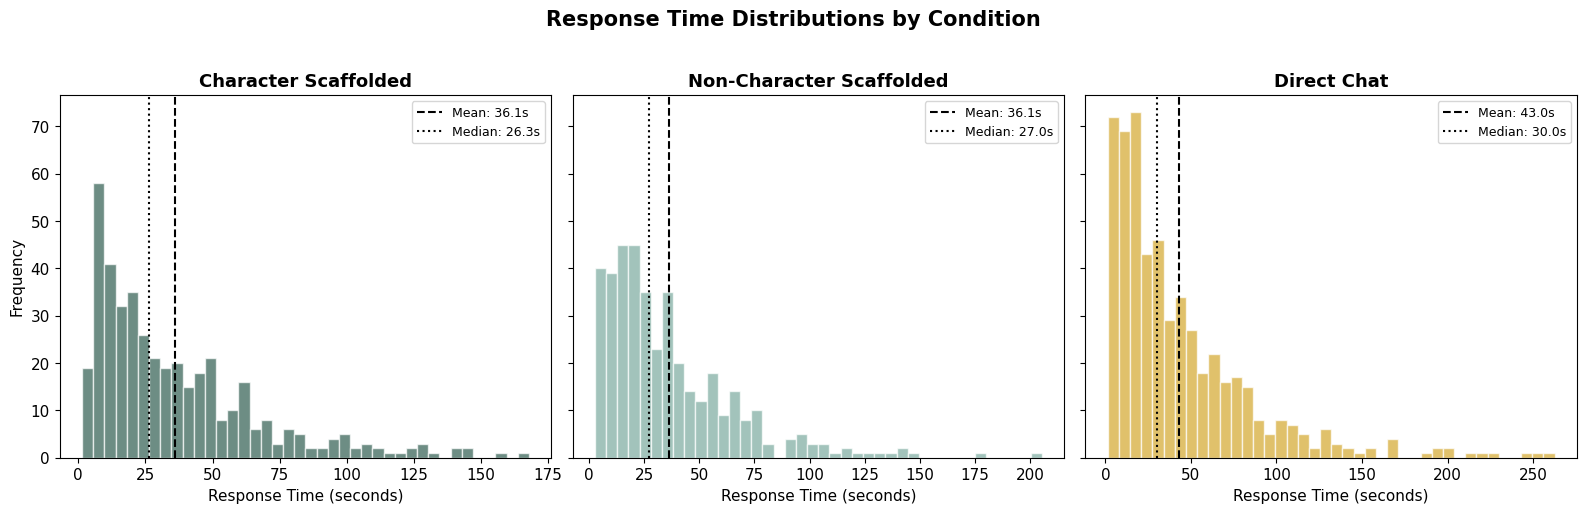
\includegraphics[width=0.9\textwidth]{sci_comp_figures/rt_distributions_2.png}
\caption{Response time distributions by condition.}
\label{fig:dist}
\end{figure}


To examine how pacing evolves within a session, response times were averaged within ten equal segments of session progress. Figure~\ref{fig:trajectory} shows the mean response-time trajectory across normalized session progress. Scaffolded conditions tend to decrease or remain stable, while direct chat drifts upward.

These trajectories suggest that scaffolding does more than accelerate responses: it 
creates a structured interaction rhythm that students can settle into. The downward 
slopes in scaffolded conditions indicate increasing fluency and reduced cognitive 
load as students progress through guided steps. In contrast, the upward drift in 
direct chat suggests accumulating friction, where students slow down as they navigate 
an unstructured conversational space.



\begin{figure}[H]
\centering
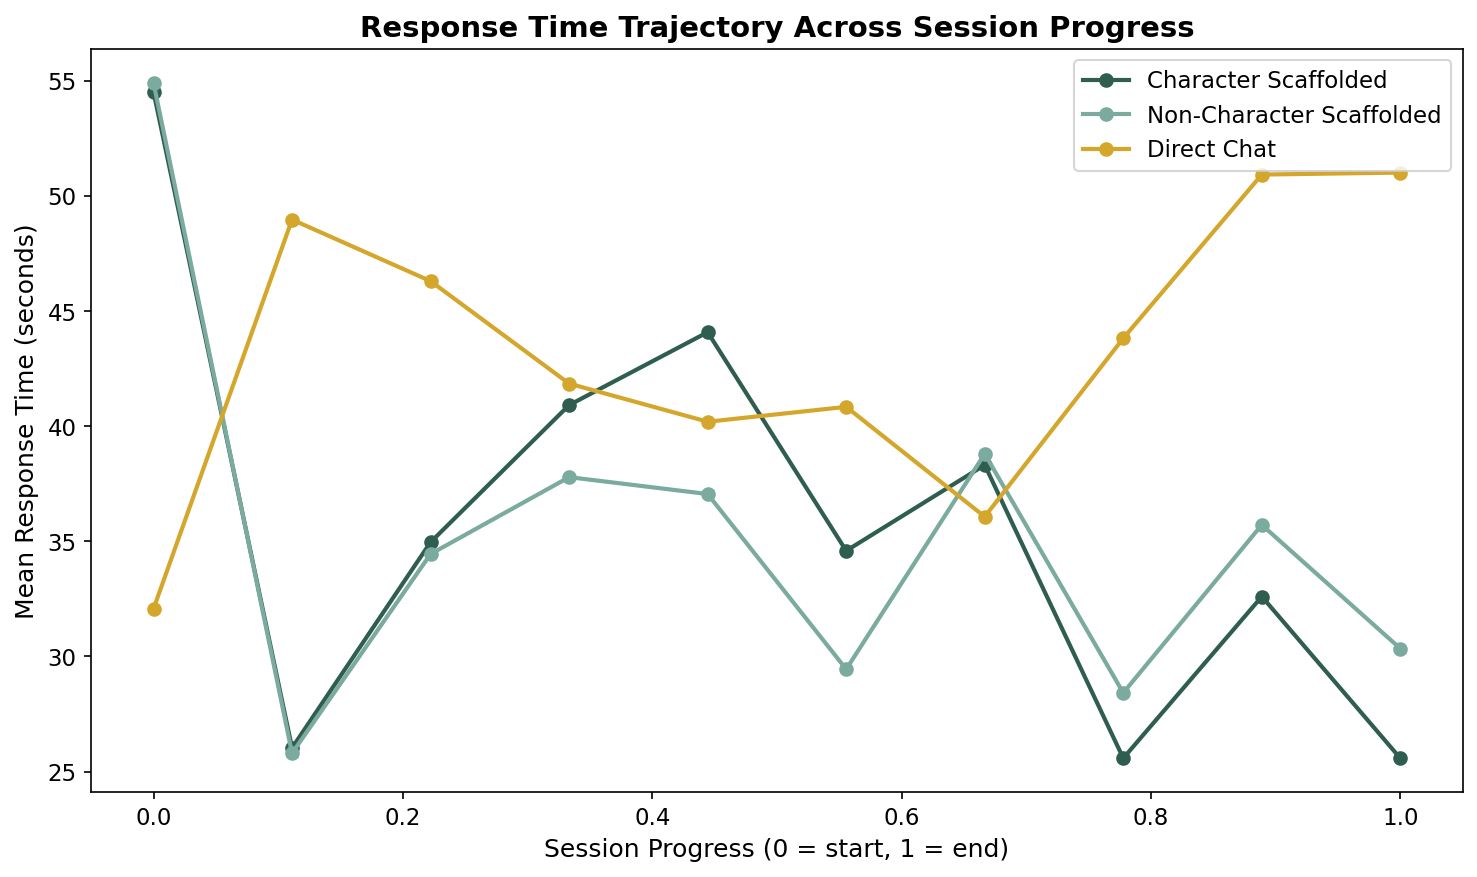
\includegraphics[width=0.60\textwidth]{sci_comp_figures/rt_trajectory.png}
\caption{Mean response time trajectory across session progress (0 = start, 1 = end).}
\label{fig:trajectory}
\end{figure}

\subsection{Bootstrap Mean Difference}

Bootstrap analysis showed that scaffolded students responded approximately 20 seconds faster on average than direct chat students. The 95\% confidence interval was [-31.79, -8.89], which excludes zero. This indicates a stable and meaningful difference in pacing (Figure~\ref{fig:bootstrap}). This confirms that the faster pacing observed in scaffolded sessions is not an artifact of sample variability but a reliable behavioral difference across the population of sessions.
\vspace{-.8em}
\begin{figure}[H]
\centering
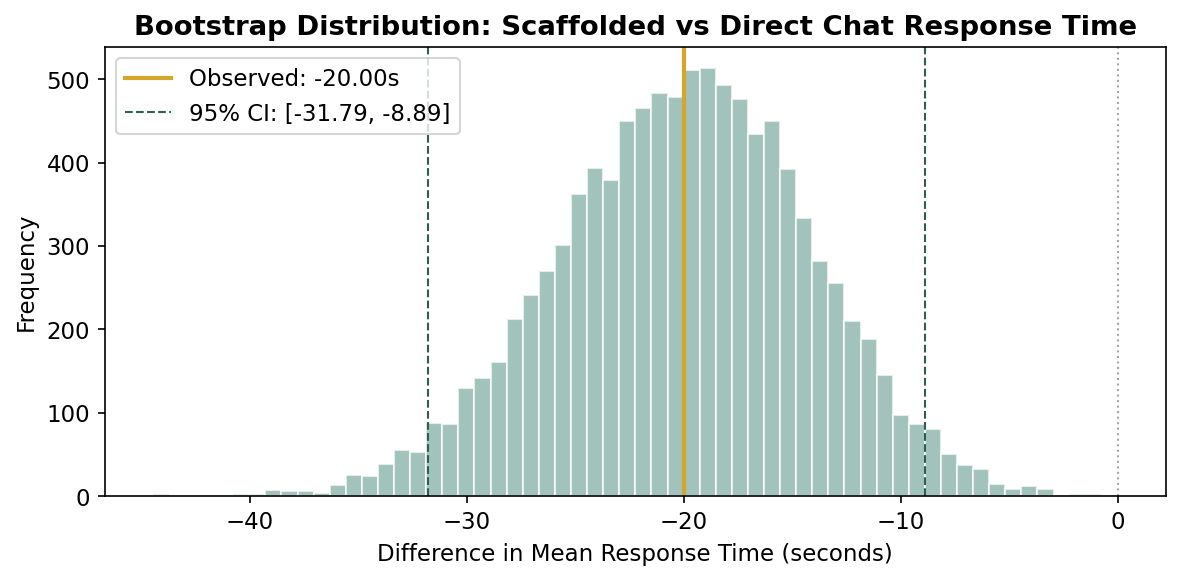
\includegraphics[width=0.5\textwidth]{sci_comp_figures/bootstrap_rt_diff.png}
\vspace{-.8em}
\caption{Bootstrap distribution of the difference in mean response time (scaffolded minus direct chat).}
\label{fig:bootstrap}
\end{figure}

\subsection{Within-Session Slopes and Local Structure}

The distribution of slopes is shown in Figure~\ref{fig:slopes}. Scaffolded sessions exhibited negative slopes (Character: -1.90 s/msg; Non-Character: -1.96 s/msg), indicating acceleration. Direct chat sessions exhibited a positive slope (+5.07 s/msg), indicating slowing down. The divergence in slopes reflects two distinct engagement dynamics:
\begin{itemize}
    \item Scaffolded sessions promote momentum: once students enter the guided sequence, their pacing tightens and becomes more efficient.
    \item  Direct chat sessions show the opposite pattern, 
with students decelerating as the session unfolds, consistent with increasing 
uncertainty or cognitive fatigue in the absence of structured prompts.
\end{itemize}


\begin{figure}[H]
\centering
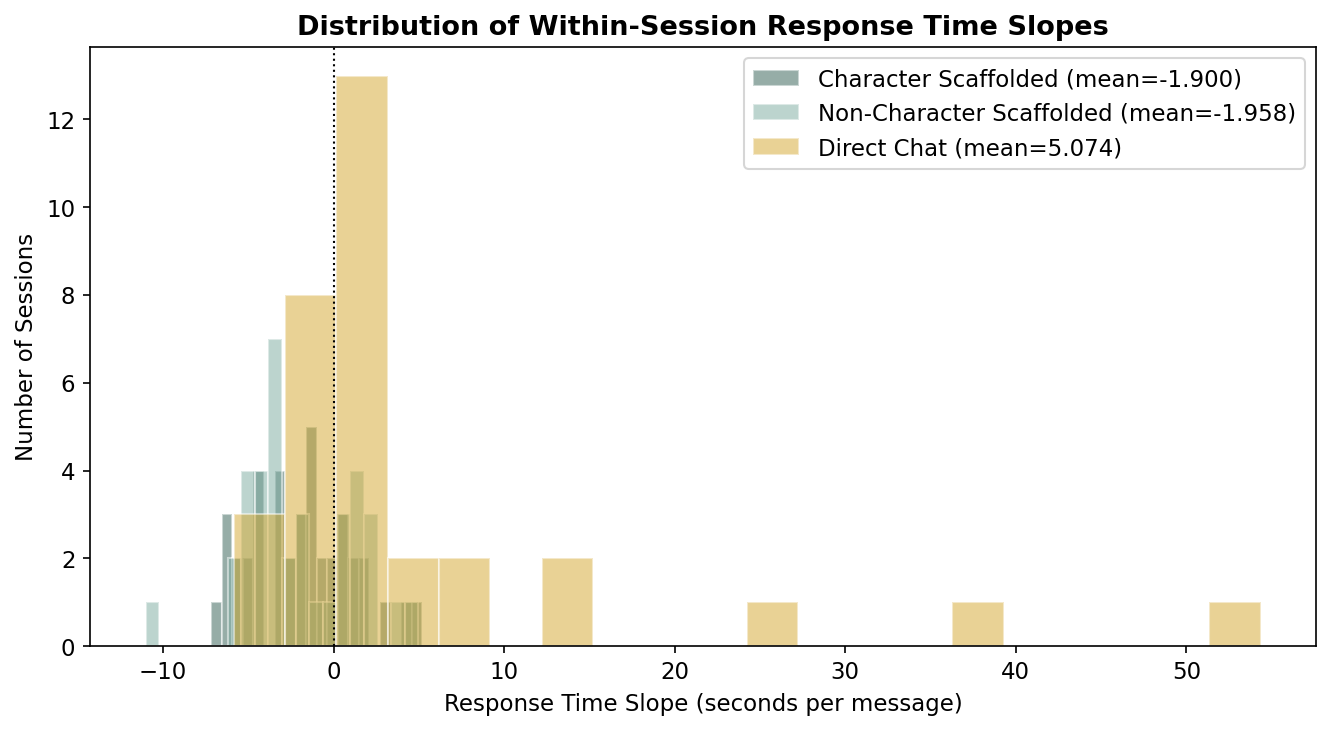
\includegraphics[width=0.6\textwidth]{sci_comp_figures/rt_slopes_distribution.png}
\caption{Distribution of within-session response-time slopes by condition.}
\label{fig:slopes}
\end{figure}

\subsection{Moving Average Smoothing}

Example sessions with raw response times, a 3-point moving average, and fitted trend 
lines are shown in Figure~\ref{fig:smoothing}. The smoothed curves reveal structure 
that is difficult to see in the noisy raw signal. Scaffolded sessions show a clear 
downward trajectory, with the moving average tightening around a stable rhythm as the 
session progresses. This pattern suggests that students settle into the guided 
sequence and gain fluency over time. In contrast, direct chat sessions show an 
upward drift even after smoothing, indicating that the slowing trend is not a 
momentary fluctuation but a persistent loss of momentum. The moving average thus 
highlights the underlying pacing dynamics that distinguish structured guidance from 
open-ended interaction.


\begin{figure}[H]
\centering
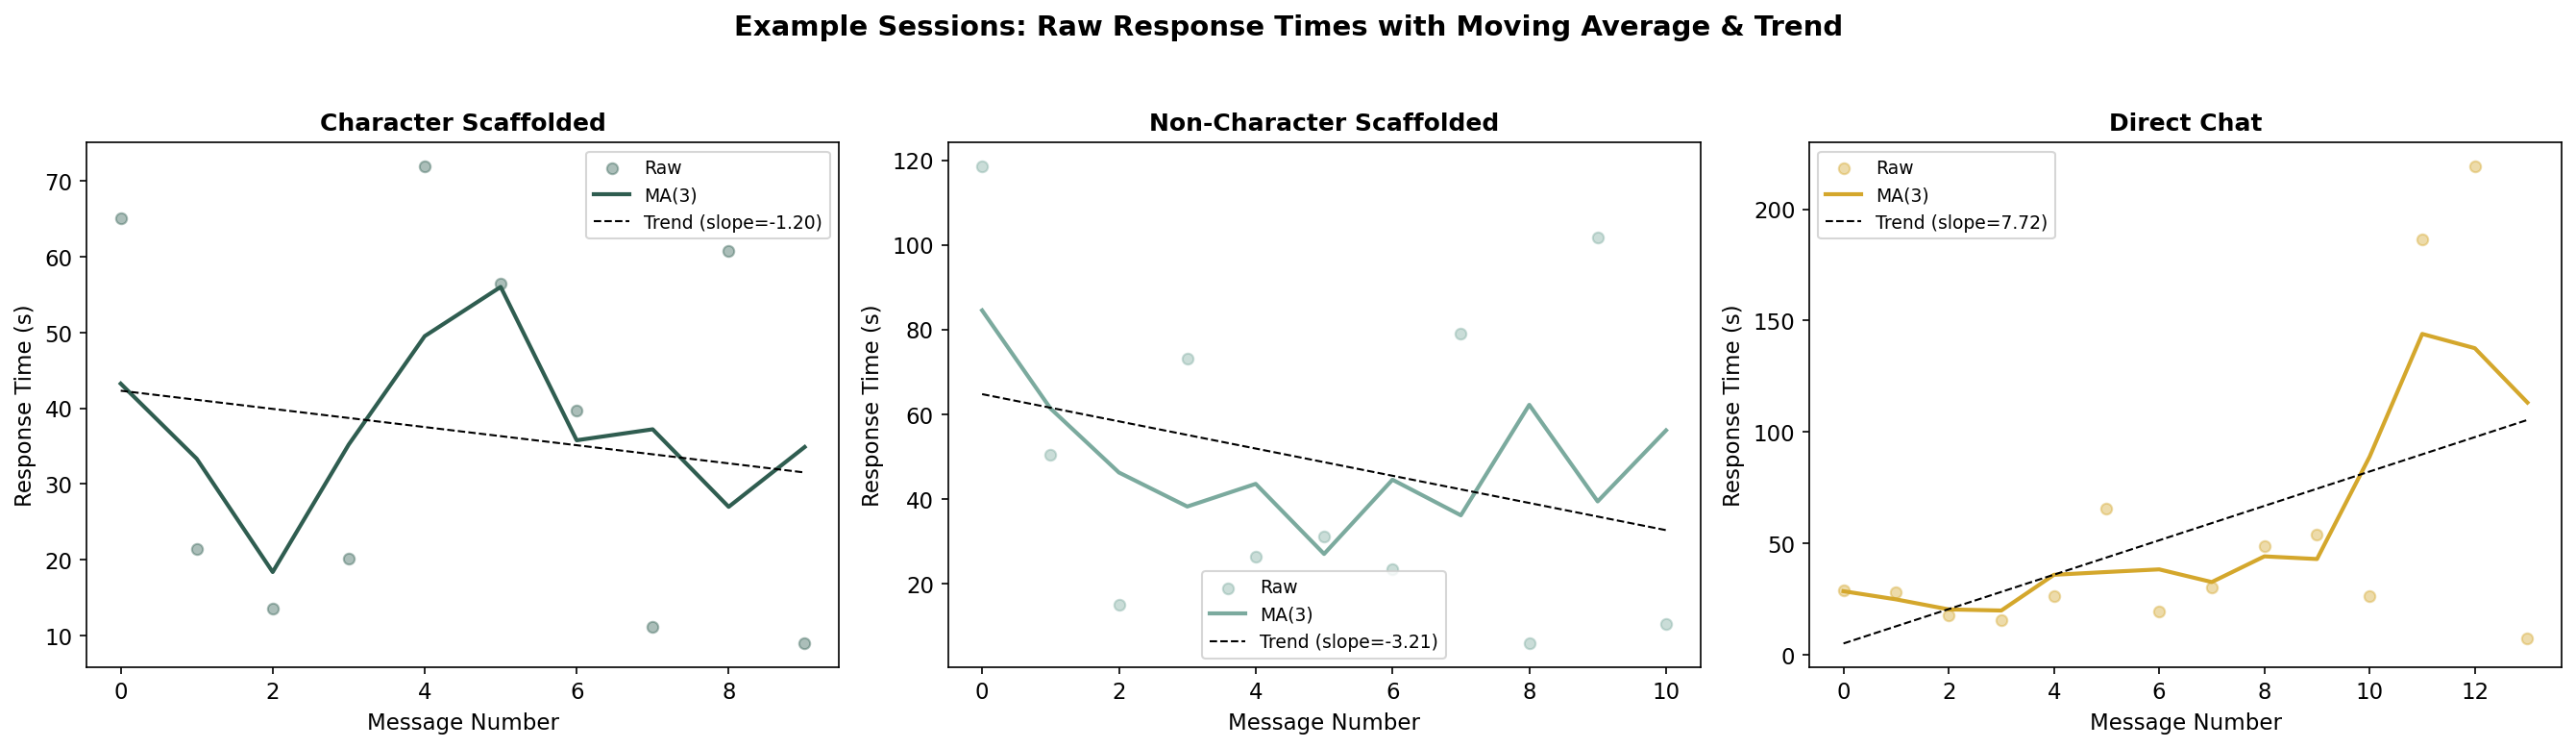
\includegraphics[width=0.75\textwidth]{sci_comp_figures/rt_smoothing_examples-2.png}
\caption{Example sessions: raw response times with moving average smoothing and linear trend.}
\label{fig:smoothing}
\end{figure}



\subsection{Frequency Structure}

FFT revealed a clear structural difference. Direct chat sessions had a dominant low-frequency spike, indicating a single monotone trend. Scaffolded sessions showed distributed energy across multiple frequencies, consistent with the structured 7-step instructional sequence of the tutor's design. The average spectra are shown in Figure~\ref{fig:fft}.

The frequency structure reinforces this interpretation. Multiple frequencies in 
scaffolded sessions indicate alternating phases of rapid and reflective engagement, 
a pattern consistent with stepwise instructional design. The single low-frequency 
component in direct chat reflects a monotonic drift rather than coordinated 
engagement cycles. Put simply, scaffolding creates a stable engagement rhythm, while direct chat gradually loses structure and momentum.


\begin{figure}[H]
\centering
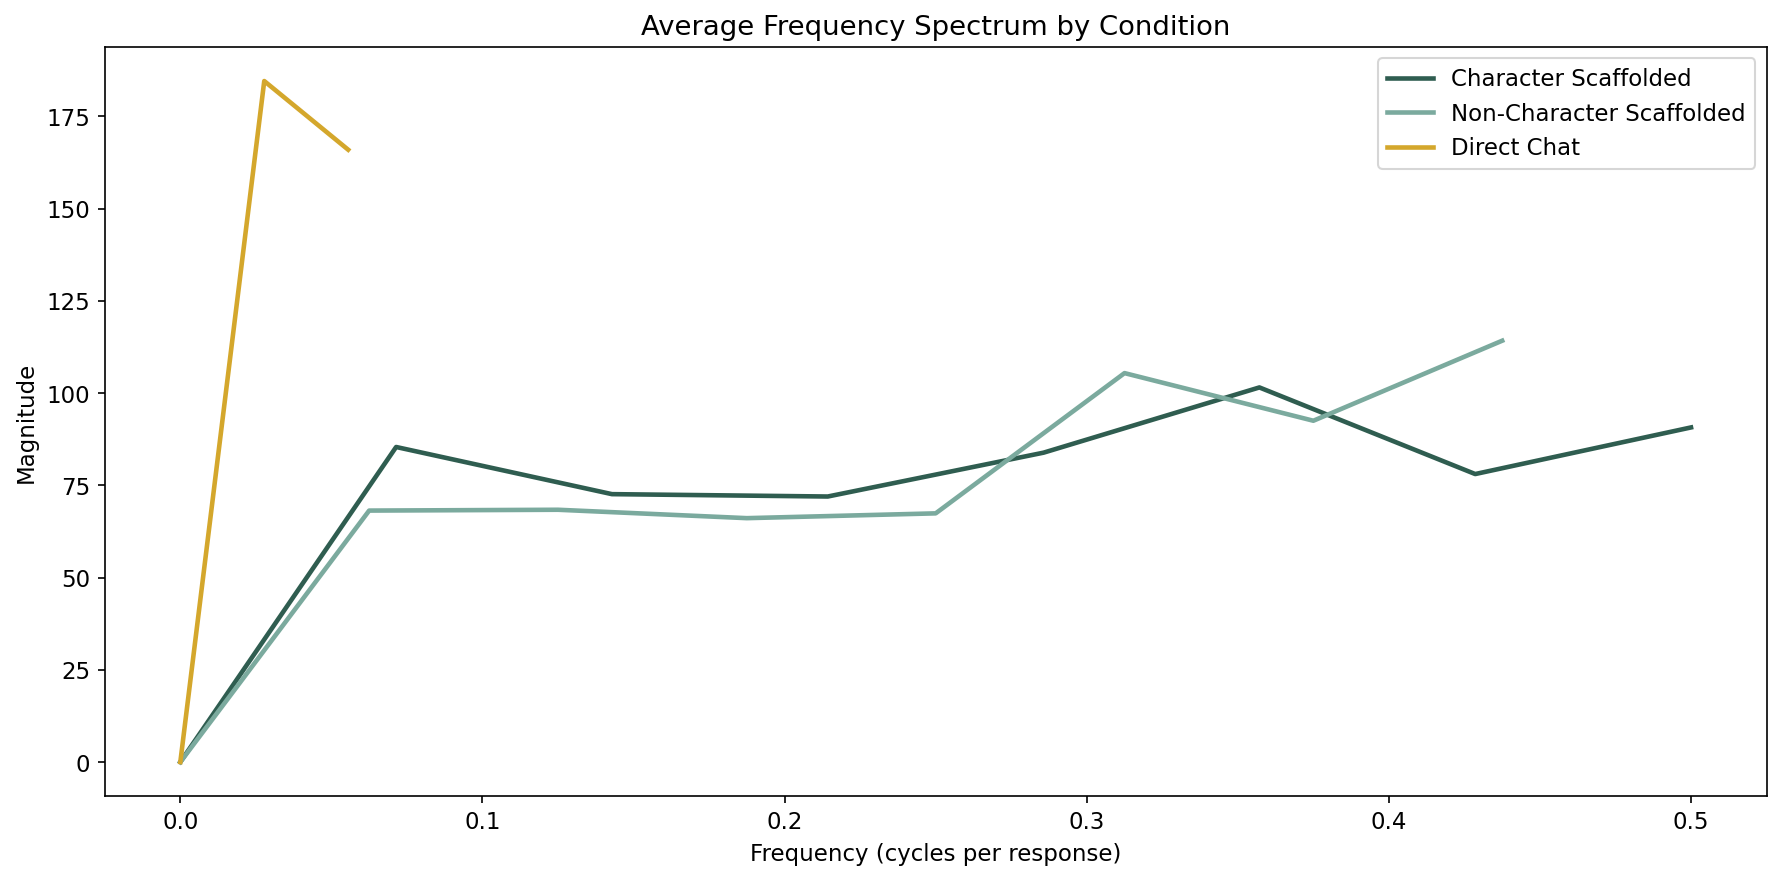
\includegraphics[width=0.6\textwidth]{sci_comp_figures/fft_by_condition.png}
\caption{Average frequency spectrum of response times by condition.}
\label{fig:fft}
\end{figure}


\section{Discussion}


This study reframes AI tutor interaction logs as a source of temporal behavioral data, emphasizing not only how much students engage, but how that engagement is structured. The results suggest that interaction rhythm -- capturing the pacing and consistency of responses—provides meaningful insight into student learning behavior.

A key finding is that interaction \textit{structure} may be as important as interaction \textit{volume}. Two students may exchange a similar number of messages or spend comparable time within a session, yet differ substantially in how that interaction is distributed. Students who exhibit steady, deliberate rhythms tend to perform better, while those with irregular or bursty patterns are more likely to struggle. This suggests that consistent pacing may reflect more effective cognitive processing, whereas erratic interaction may indicate guessing, confusion, or disengagement.

Computationally, these rhythm features are easy to interpret, especially compared to more opaque modeling approaches. Rather than relying solely on aggregate engagement metrics or correctness-based signals, this framework captures temporal dynamics directly observable in interaction logs. This also makes the approach practical for real‑time use in AI tutoring systems.

These patterns matter for adaptive learning systems in practice. Since rhythm shows up in real time, an AI tutor could actually react to it: adjusting support when a student speeds up, slows down, or gets stuck. For example, bursts of rapid responses might trigger reflective prompts, while extended inactivity could prompt additional scaffolding or guidance.

\subsection{Limitations}

This study is based on a relatively small dataset from a single programming course, which may limit generalizability. Additionally, rhythm is captured using session-level aggregate features, which do not fully represent sequential interaction dynamics. Future work could explore more detailed temporal modeling approaches to capture finer-grained behavioral patterns.


\section{Conclusion}

This project demonstrates that response times, treated as time-series signals, contain meaningful behavioral information about engagement. Scaffolded sessions are faster, more stable, and more structured. Direct chat sessions slow down and show a single dominant temporal trend. Time-series methods reveal patterns that are invisible in aggregate statistics and highlight the value of analyzing the temporal structure of human-AI interactions.


\footnotesize

\begin{thebibliography}{9}


\bibitem{twitter2023}
Mayor, E., Bietti, L. M., and Canales-Rodr{\'i}guez, E. J. 
\textit{Text as signal: A tutorial with case studies focusing on social media (Twitter)}. 
Behavior Research Methods, 55(5), 2595--2620, 2023. 
doi: 10.3758/s13428-022-01917-1.

\bibitem{papadogiannis2024}
Papadogiannis, I., Wallace, M., and Karountzou, G.
``Educational Data Mining: A Foundational Overview.''
\textit{Encyclopedia}, 4(4), 1644--1664, 2024.
doi: 10.3390/encyclopedia4040108.


\end{thebibliography}
\vspace{-1em}

\end{document}
